\chapter{Results}
\label{ch:results}

\begin{quote}
\textbf{Note.} This chapter presents the empirical results of the measurement campaign described in Chapter~\ref{ch:method}. The campaign spans 50 days in total (2 April -- 21 May 2026), comprising a pilot phase (2--10 April, 99 domains, 50 probes per measurement) and a main phase (11 April -- 21 May, 248 domains, 200 probes per measurement). The quantitative results reported here are based on the first 45 days of data collected (2 April -- 16 May 2026); all statistics will be finalized upon campaign completion on 21 May 2026.
\end{quote}

\bigskip
\section{Dataset Overview}
\label{sec:4.1}

\subsection{Collection Statistics}
\label{subsec:4.1.1}

The measurement campaign began on 2 April 2026. Two phases are combined in the dataset: a pilot phase (2--10 April) using 99 domains and 50 probes per measurement, and a main phase (11 April -- 21 May) using 248 domains and 200 probes per measurement. The main-phase corpus overlaps almost entirely with the pilot corpus, extending it by an additional 149 domains. Table~\ref{tab:4.1} summarises the collection statistics for the first 45 days (2 April -- 16 May 2026) currently available.

\begin{table}[H]
\centering
\small
\begin{tabular}{l l}
\toprule
\textbf{Metric} & \textbf{Value} \\
\midrule
Measurement period & 2 April 2026 -- 21 May 2026 (50 days total; statistics from first 45 days) \\
Domains monitored & 248 (99 during pilot, 248 during main phase) \\
Unique RIPE Atlas probe IDs observed & 10,862 \\
Countries covered & 173 \\
Total \ac{DNS} measurement results retrieved & 1,564,904 \\
Results with RCODE = NOERROR & 1,505,890 (96.2\%) \\
Results with RCODE = REFUSED & 14,628 (0.9\%) \\
Results with RCODE = SERVFAIL & 10,118 (0.6\%) \\
Results with no response (timeout / no \texttt{abuf}) & 31,395 (2.0\%) \\
Results with RCODE = FORMERR & 2,559 (0.2\%) \\
Results with RCODE = NXDOMAIN & 314 (0.0\%) \\
Results with \ac{NSID} present & 812,185 (51.9\%) \\
Mean \ac{RTT} across all valid results & 71.34 ms \\
\bottomrule
\end{tabular}
\caption{Campaign summary statistics (50-day campaign, 2 April -- 21 May 2026; values from the first 45 days, 2 April -- 16 May 2026)}
\label{tab:4.1}
\end{table}

The 96.2\% valid result rate (RCODE=0) slightly exceeds the 85--90\% conservative estimate from Chapter~\ref{ch:method}, consistent with the high-reliability authoritative infrastructure of Tranco Top 250 domains. The 2.0\% no-response rate is attributable to probes that went offline between measurement scheduling and execution or experienced transient connectivity failures. The 0.9\% REFUSED rate reflects a small number of authoritative servers that block queries originating from RIPE Atlas probe addresses; these results are excluded from all subsequent analyses.

Across the 45-day partial period (2 April -- 16 May 2026), 10,862 unique probe IDs appear in the dataset. This figure reflects the fact that the campaign runs one independent RIPE Atlas measurement per domain: 99 parallel measurements during the pilot (each with 50 probes) and 248 during the main phase (each with 200 probes). Because each measurement is assigned its own probe set independently, the total number of probe appearances is approximately $99 \times 50 + 248 \times 200 = 54{,}550$, and the union of all probe IDs across those assignments yields 10,862 unique identifiers. Each probe ID appears on average in roughly five different domain measurements, consistent with RIPE Atlas area-based probe assignment, which independently draws probe sets from the same geographic zones for each measurement, causing widely-available probes (e.g., in Germany or the United States) to appear across many domain measurements.

\subsection{Probe Distribution}
\label{subsec:4.1.2}

Table~\ref{tab:4.2} reports the geographic distribution of the 10,862 unique probe IDs by continent. Europe accounts for 57.8\% of probes and North America for 21.2\%, together representing 79.0\% of all unique probe IDs. Asia-Pacific contributes 12.4\%. Africa (2.0\%), Oceania (3.2\%), and South America (3.4\%) are substantially under-represented relative to their share of global Internet users. Section~\ref{sec:4.4} analyses the impact of this distribution on the measurement results.

\begin{table}[H]
\centering
\small
\begin{tabular}{l r r r r}
\toprule
\textbf{Continent} & \textbf{Unique probe IDs} & \textbf{Share (\%)} & \textbf{Countries covered} & \textbf{Avg.\ probes/country} \\
\midrule
Europe          & 6,278 & 57.8\% & 44  & 142.7 \\
North America   & 2,299 & 21.2\% & 13  & 176.8 \\
Asia-Pacific    & 1,343 & 12.4\% & 63  &  21.3 \\
South America   &   374 &  3.4\% & 10  &  37.4 \\
Oceania         &   350 &  3.2\% &  8  &  43.8 \\
Africa          &   218 &  2.0\% & 35  &   6.2 \\
\textbf{Total}  & \textbf{10,862} & \textbf{100\%} & \textbf{173} & \textbf{62.8} \\
\bottomrule
\end{tabular}
\caption{Geographic distribution of unique probe IDs by continent (50-day campaign, 2 April -- 21 May 2026; data from first 45 days). ``Countries covered'' is the number of distinct countries contributing at least one probe; ``Avg.\ probes/country'' is the ratio of unique probe IDs to countries covered, reflecting sampling density.}
\label{tab:4.2}
\end{table}

Despite using RIPE Atlas geographic zone-based probe selection, the actual probe distribution is still Europe-heavy. This reflects the structural composition of the RIPE Atlas probe network, in which approximately 60\% of connected probes are located in Europe~\cite{Bajpai2017}. Across the 247 independent measurements, RIPE Atlas assigned probes from 173 countries in total, including 34 countries with a single probe and 139 countries with multiple probes, but the fundamental scarcity of probes in Africa, South America, and Oceania cannot be overcome by selection alone.

\subsection{Data Quality}
\label{subsec:4.1.3}

The domain coverage is complete: analysis tools processed measurements for 247 of the 248 domains in the corpus (one domain produced no valid results across the entire campaign period and was excluded from per-domain analyses). Coverage per continent is 99.6\% for all six continental regions, confirming that all continents are represented for virtually every domain.

The mean \ac{RTT} across the 45-day partial period is 71.34 ms. The pilot phase (2--10 April, 50 probes) yields an average of 60.15 ms, while the main phase (11 April -- 21 May, 200 probes) yields 71.67 ms based on the first 36 days available. The higher \ac{RTT} in the main phase is consistent with the larger and more geographically dispersed probe set, which includes a greater proportion of probes in high-latency regions such as Africa and Oceania.

\bigskip
\section{Results for Q1: Geographic Diversity of DNS Responses}
\label{sec:4.2}

\textbf{Research question}: What proportion of popular domains return geographically differentiated DNS responses, and what infrastructure mechanisms explain the differentiation?

\subsection{Overall Distribution of Geographic Diversity}
\label{subsec:4.2.1}

The analysis operates at two geographic granularities: continent-level (six groups) and country-level (173 countries). At the continent level, a domain is classified as geographically diverse if the set of \ac{IP} addresses observed by probes from at least two different continents differs on at least one measurement day. At the country level, the same criterion is applied across country groups.

Under these criteria, 148 of 247 domains (59.9\%) exhibit geographic diversity at the continent level, and 149 of 247 domains (60.3\%) exhibit geographic diversity at the country level. The near-identical rates at the two granularities indicate that intra-continental diversity (variation between countries within the same continent) is pervasive: virtually every continent-diverse domain also exhibits measurable intra-continental variation.

The mean number of distinct \ac{IP} address sets observed across continental probe groups is 2.67 per domain (continent-level) and 11.45 per domain (country-level). The substantially higher country-level figure reflects the fine-grained routing differentiation practised by major \ac{CDN} operators, which may serve distinct \ac{IP} pools to individual countries or metropolitan regions even within the same continent.

The 99 remaining domains (40.1\%) returned a consistent set of \ac{IP} addresses across all probe groups. These are predominantly smaller or single-homed services not deploying \ac{CDN} or anycast infrastructure.

\begin{figure}[H]
\centering
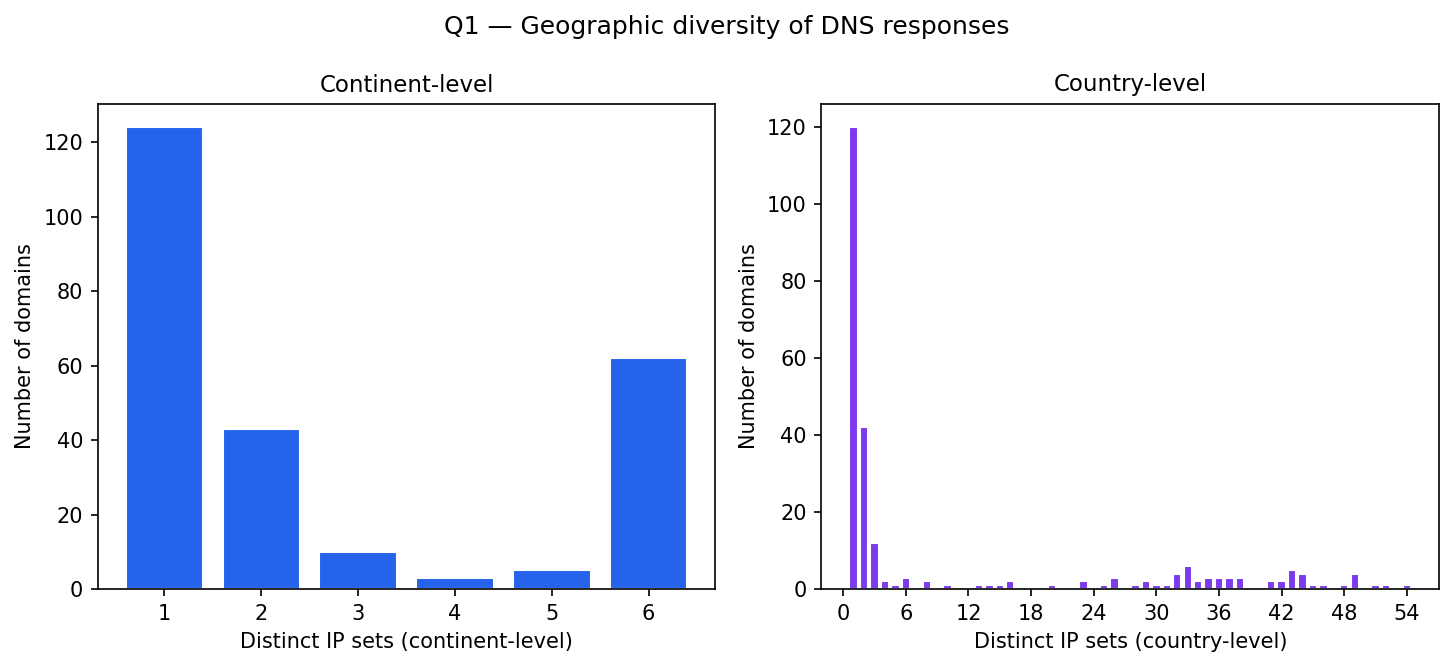
\includegraphics[width=0.85\textwidth]{figures/fig_q1a_ip_set_diversity.png}
\caption{Distribution of the number of distinct \ac{IP} address sets per domain, at two geographic granularities (50-day campaign, 45-day partial data, 247 domains). \textit{Top}: continent-level --- a value of 1 indicates a uniform response across all six continental probe groups; values above 1 indicate cross-continental differentiation. \textit{Bottom}: country-level --- the long tail reflects fine-grained \ac{CDN} routing that differentiates responses at the individual country level.}
\label{fig:q1a}
\end{figure}

\begin{figure}[H]
\centering
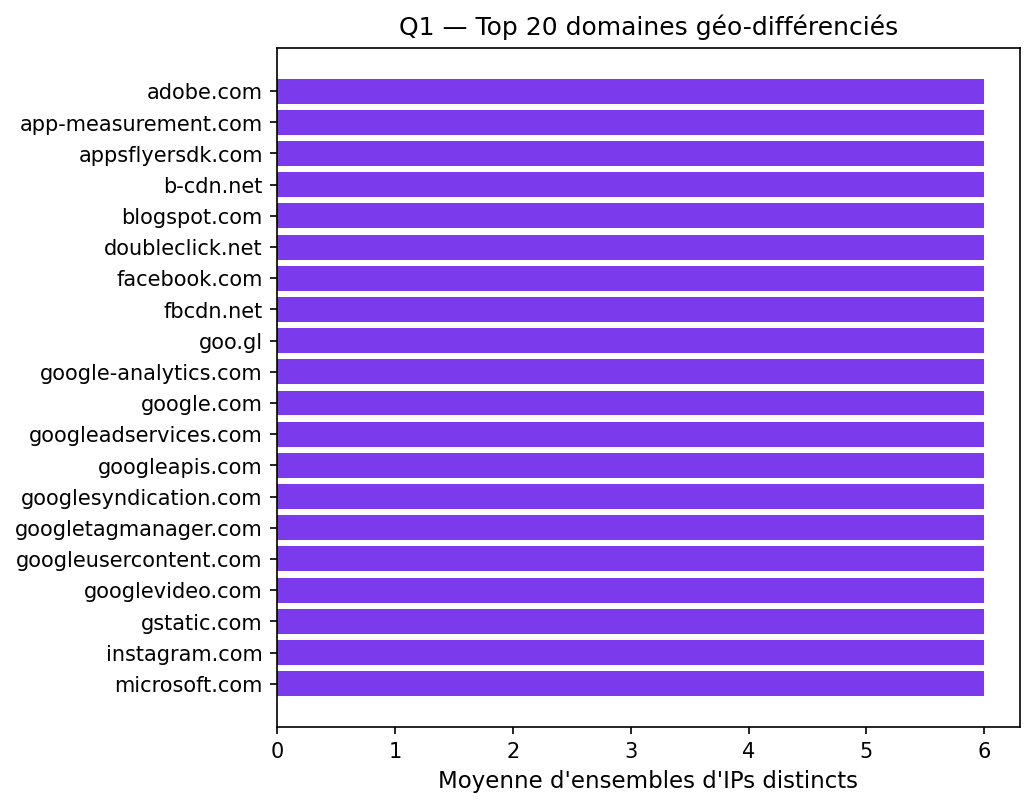
\includegraphics[width=0.85\textwidth]{figures/fig_q1b_top20_geo_diverse.png}
\caption{Top 20 most geographically diverse domains, ranked by mean number of distinct \ac{IP} address sets observed at the country level. Values annotated on each bar are the mean count over the 45-day partial dataset (50-day campaign).}
\label{fig:q1b}
\end{figure}

\subsection{NSID as an Anycast Indicator}
\label{subsec:4.2.2}

Of the 247 analysed domains, 191 (77.3\%) have at least one measurement result carrying an \ac{NSID} string in the OPT record of the \ac{DNS} response. \ac{NSID} is inserted by authoritative servers to identify the specific anycast instance that answered the query (\cite{RFC5001}); its presence is a strong indicator of anycast-based authoritative \ac{DNS} deployment. The high \ac{NSID} rate (77.3\% at the domain level; 51.9\% at the measurement-result level) confirms that anycast-based routing is the predominant infrastructure mechanism underlying geographic \ac{DNS} differentiation in the Tranco Top 250 corpus.

The \ac{NSID} presence rate differs between the two groups: 56.6\% of measurement results for continent-diverse domains carry an \ac{NSID} string, versus 47.3\% for uniform domains. This difference is consistent with the hypothesis that anycast infrastructure drives geographic \ac{DNS} response variation by directing queries to the physically nearest authoritative instance --- domains with anycast deployment both expose their instance identity via \ac{NSID} and return different \ac{IP}s to different regions.

\subsection{Interpretation}
\label{subsec:4.2.3}

The 59.9\% continent-level geographic diversity rate among the Tranco Top 250 is consistent with the \ac{CDN}-heavy composition of the top-ranked domains: major web properties served by Cloudflare, Akamai, Fastly, or Amazon CloudFront routinely return different \ac{IP} pools to different geographic regions. The jump from a mean of 2.67 distinct \ac{IP} sets at the continent level to 11.45 at the country level (Section~\ref{subsec:4.2.1}) indicates that \ac{CDN} operators do not simply route by continental region: they maintain fine-grained routing tables that differentiate responses at the individual country level or below.

The 50-day campaign (with 45 days of data currently available) provides a more reliable estimate of geographic diversity than the 9-day pilot phase alone: \ac{CDN} routing policies that change slowly (e.g., weekly pool rotations) are now well captured within the observation period. The remaining uncertainty is that domains with \ac{DNS}-level \ac{CDN} routing driven primarily by \ac{ECS} (Section~\ref{subsec:3.3.4}) may exhibit diversity patterns visible at the resolver level but not at the probe level, since RIPE Atlas probes use their local \ac{ISP} resolver which may or may not forward \ac{ECS} to authoritative servers.

\bigskip
\section{Results for Q2: Temporal Stability}
\label{sec:4.3}

\textbf{Research question}: What is the temporal stability of DNS responses for popular domains over day, week, and month timescales?

\subsection{Aggregate Change Rate}
\label{subsec:4.3.1}

For each (domain, probe) pair, the temporal change rate is defined as the fraction of consecutive daily measurement pairs for which the observed \ac{IP} address set changed. Table~\ref{tab:4.3} reports the aggregate change rate computed over three temporal windows: daily (consecutive-day pairs), weekly (pairs seven days apart), and monthly (pairs 30 days apart).

\begin{table}[H]
\centering
\small
\begin{tabular}{l r l}
\toprule
\textbf{Window} & \textbf{Change rate} & \textbf{Note} \\
\midrule
Daily   & 38.24\% & 44 consecutive-day pairs available \\
Weekly  & 38.29\% & 38 seven-day pairs available \\
Monthly & 38.30\% & 15 pairs available \\
\bottomrule
\end{tabular}
\caption{\ac{DNS} response change rates by temporal window (partial dataset: 2 April -- 16 May 2026; campaign total: 50 days, ending 21 May 2026)}
\label{tab:4.3}
\end{table}

The near-identical values across all three windows (38.24\%, 38.29\%, 38.30\%) indicate that the dominant change mechanism is the short-\ac{TTL} \ac{CDN} pool rotation that operates continuously, rather than episodic infrastructure events (server migrations, \ac{IP} address reallocations) that would produce a step change visible at longer timescales. In other words, a (domain, probe) pair that changes responses on consecutive days continues to change at approximately the same rate one week or one month later, suggesting a stable churn process rather than a convergent one.

With fifteen monthly comparison pairs now available, the monthly estimate of 38.30\% is well-established. The convergence of the daily, weekly, and monthly rates confirms that \ac{CDN} pool rotation behaves as a stationary process within the 50-day campaign window.

Of the 247 analysed domains, 51 (20.6\%) are classified as fully stable: their \ac{IP} address set does not change across any consecutive measurement pair within the 45-day partial observation window. The 38.24\% figure above is an aggregate rate computed across all (domain, probe, day) triplets; it is pulled down by the 20.6\% of fully stable domains that contribute zero-change pairs. The median per-domain change rate is 48.8\%, reflecting the typical behaviour of the non-stable majority: once a domain exhibits churn, it tends to change on roughly half of all daily measurement pairs.

\begin{figure}[H]
\centering
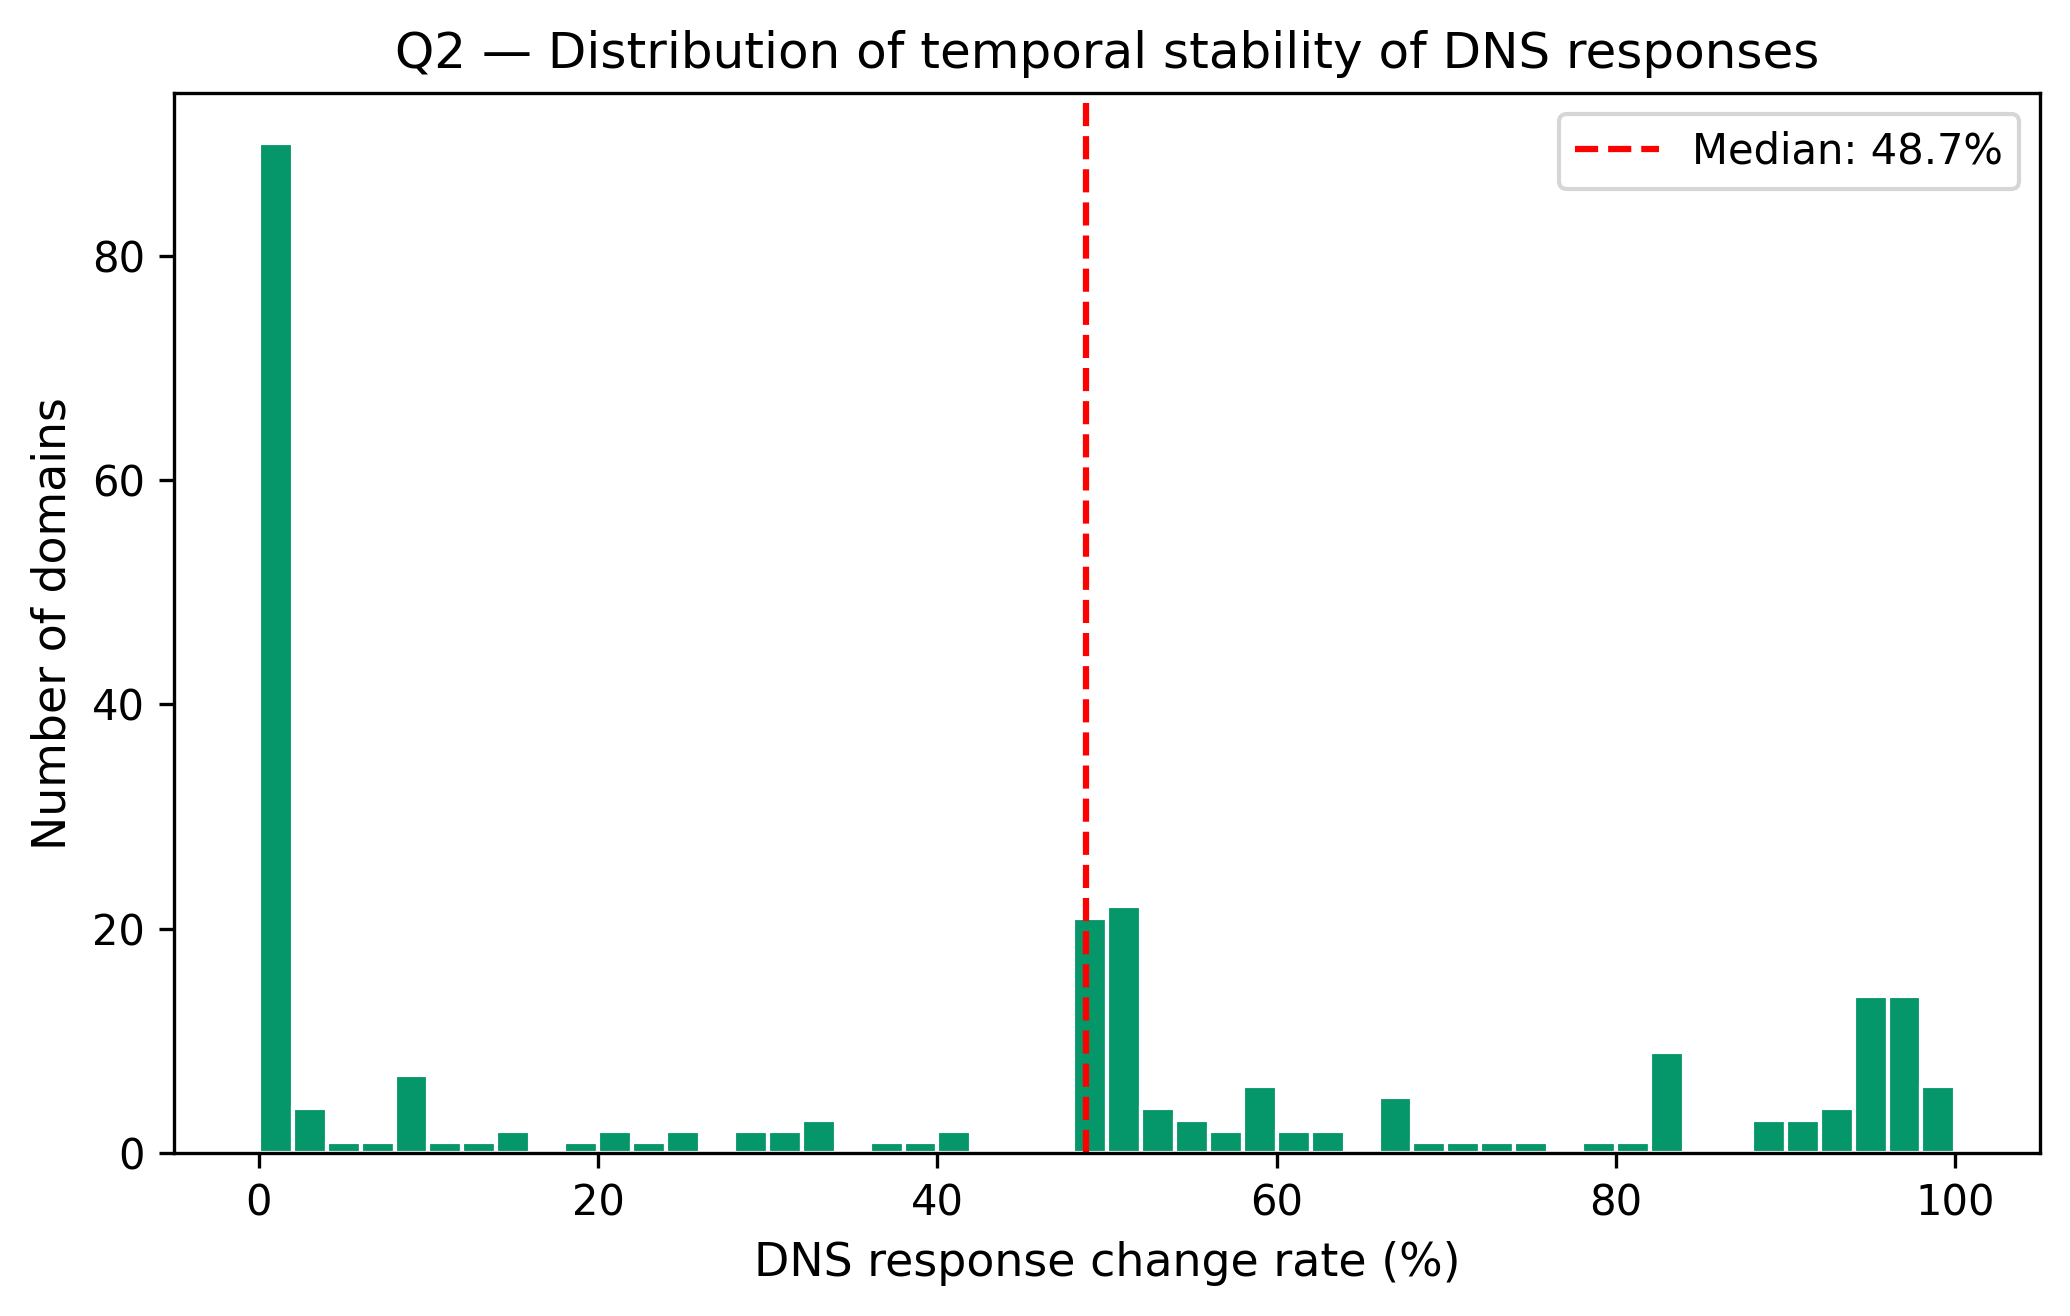
\includegraphics[width=0.85\textwidth]{figures/fig_q2_temporal_stability.png}
\caption{Distribution of per-domain \ac{DNS} response change rates over the 50-day measurement campaign (45-day partial data shown). Domains with a change rate of 0\% are fully stable (20.6\% of the corpus); the remainder show substantial daily churn, with a median of 48.8\%.}
\label{fig:q2}
\end{figure}

\subsection{Interpretation}
\label{subsec:4.3.2}

The daily change rate of 38.24\% is substantially higher than the 0.6\% daily turnover of the Tranco domain popularity ranking~\cite{LePochat2019}, confirming that \ac{DNS} response content is far more volatile than the domain popularity ordering. At approximately 64 times the list-level churn rate, this gap is expected: \ac{CDN} operators routinely configure short \ac{TTL}s (60--300 seconds for major providers) to enable rapid traffic redistribution across server pools, and RIPE Atlas probes that bypass the recursive resolver cache by querying authoritative servers directly will observe a new \ac{IP} set at each daily measurement with probability proportional to the pool rotation rate.

The bimodal character of the distribution --- approximately 20.6\% of domains are fully stable and the remainder show high churn --- corresponds to a structural split in the corpus. Fully stable domains are predominantly those with static, non-\ac{CDN} authoritative infrastructure (corporate intranets, government websites, small organisations); the high-churn majority are \ac{CDN}-backed services whose authoritative servers return dynamically load-balanced \ac{IP} pools.

The weekly rate (38.29\%) and monthly rate (38.30\%) are statistically indistinguishable from the daily rate (38.24\%), confirming that \ac{CDN} pool rotation is a stationary process across all three timescales: there is no systematic convergence or divergence within the 50-day campaign window. With fifteen monthly comparison pairs now available, this conclusion rests on solid empirical ground.

\bigskip
\section{Results for Q3: RIPE Atlas Geographic Bias Assessment}
\label{sec:4.4}

\textbf{Research question}: Do the documented geographic biases of the RIPE Atlas probe distribution significantly limit the ability to observe DNS geographic response variation?

\subsection{Bias in the Observed Probe Distribution}
\label{subsec:4.4.1}

The actual probe distribution (Table~\ref{tab:4.2}) shows that Europe and North America together account for 79.0\% of unique probe IDs, despite the geographic zone-based probe selection used for this campaign. In a perfectly balanced six-continent design each continent would hold approximately 16.7\% of probes; the actual EU+NA share of 79.0\% is nearly five times that target, confirming the well-documented structural concentration of RIPE Atlas in Western networks~\cite{Bajpai2017}.

The sampling density column (avg.\ probes/country) reveals the depth of the imbalance more starkly than raw counts alone: a European country contributes on average 142.7 probe IDs to the dataset, versus 6.2 for an African country. Asia-Pacific, despite contributing 63 countries (the most of any continent), averages only 21.3 probes per country, reflecting both the scarcity of RIPE Atlas probes in the region and the large number of countries it encompasses. Despite this concentration, the zone-based probe assignment covered 173 countries across all six continents, ensuring that global geographic coverage is maintained even if sampling density is unequal.

\subsection{Statistical Test of Measurement Impact}
\label{subsec:4.4.2}

To assess whether the geographic imbalance materially affects observed \ac{DNS} diversity, a Mann-Whitney U test compares the distribution of per-(domain, continent) unique \ac{IP} address counts between the Europe+North America group and all other continents (Asia-Pacific, Africa, South America, Oceania). The Mann-Whitney test is used because the \ac{IP}-set count distributions are heavily right-skewed and non-normal (as visible in Figure~\ref{fig:q1a}), making parametric tests inappropriate.

The test yields:
\[
U = 256{,}971.5, \quad p = 0.091
\]

The result is above the conventional $\alpha = 0.05$ threshold and is not statistically significant. Two interpretations are consistent with this finding: (1) \ac{CDN} infrastructure genuinely routes different \ac{IP} pools to different geographic regions, producing a real but modest distributional difference that the current dataset does not detect with certainty; (2) the Europe/NA-heavy probe set may undersample \ac{DNS} variation patterns specific to under-represented regions (Africa, South America, Oceania), partially masking any difference.

A second Mann-Whitney U test compares single-probe countries (34 countries with only one probe in the entire dataset) against multi-probe countries (139 countries with two or more probes), to assess whether country-level representativeness affects the diversity signal:
\[
U = 2{,}844{,}086.0, \quad p = 0.094
\]

This result also does not reach statistical significance at $\alpha = 0.05$. The direction of the effect is consistent with single-probe countries exhibiting higher variance in observed \ac{IP}-set counts (a single probe provides no within-country replication), but with the 45-day partial dataset the difference is not statistically distinguishable from sampling variability.

\begin{figure}[H]
\centering
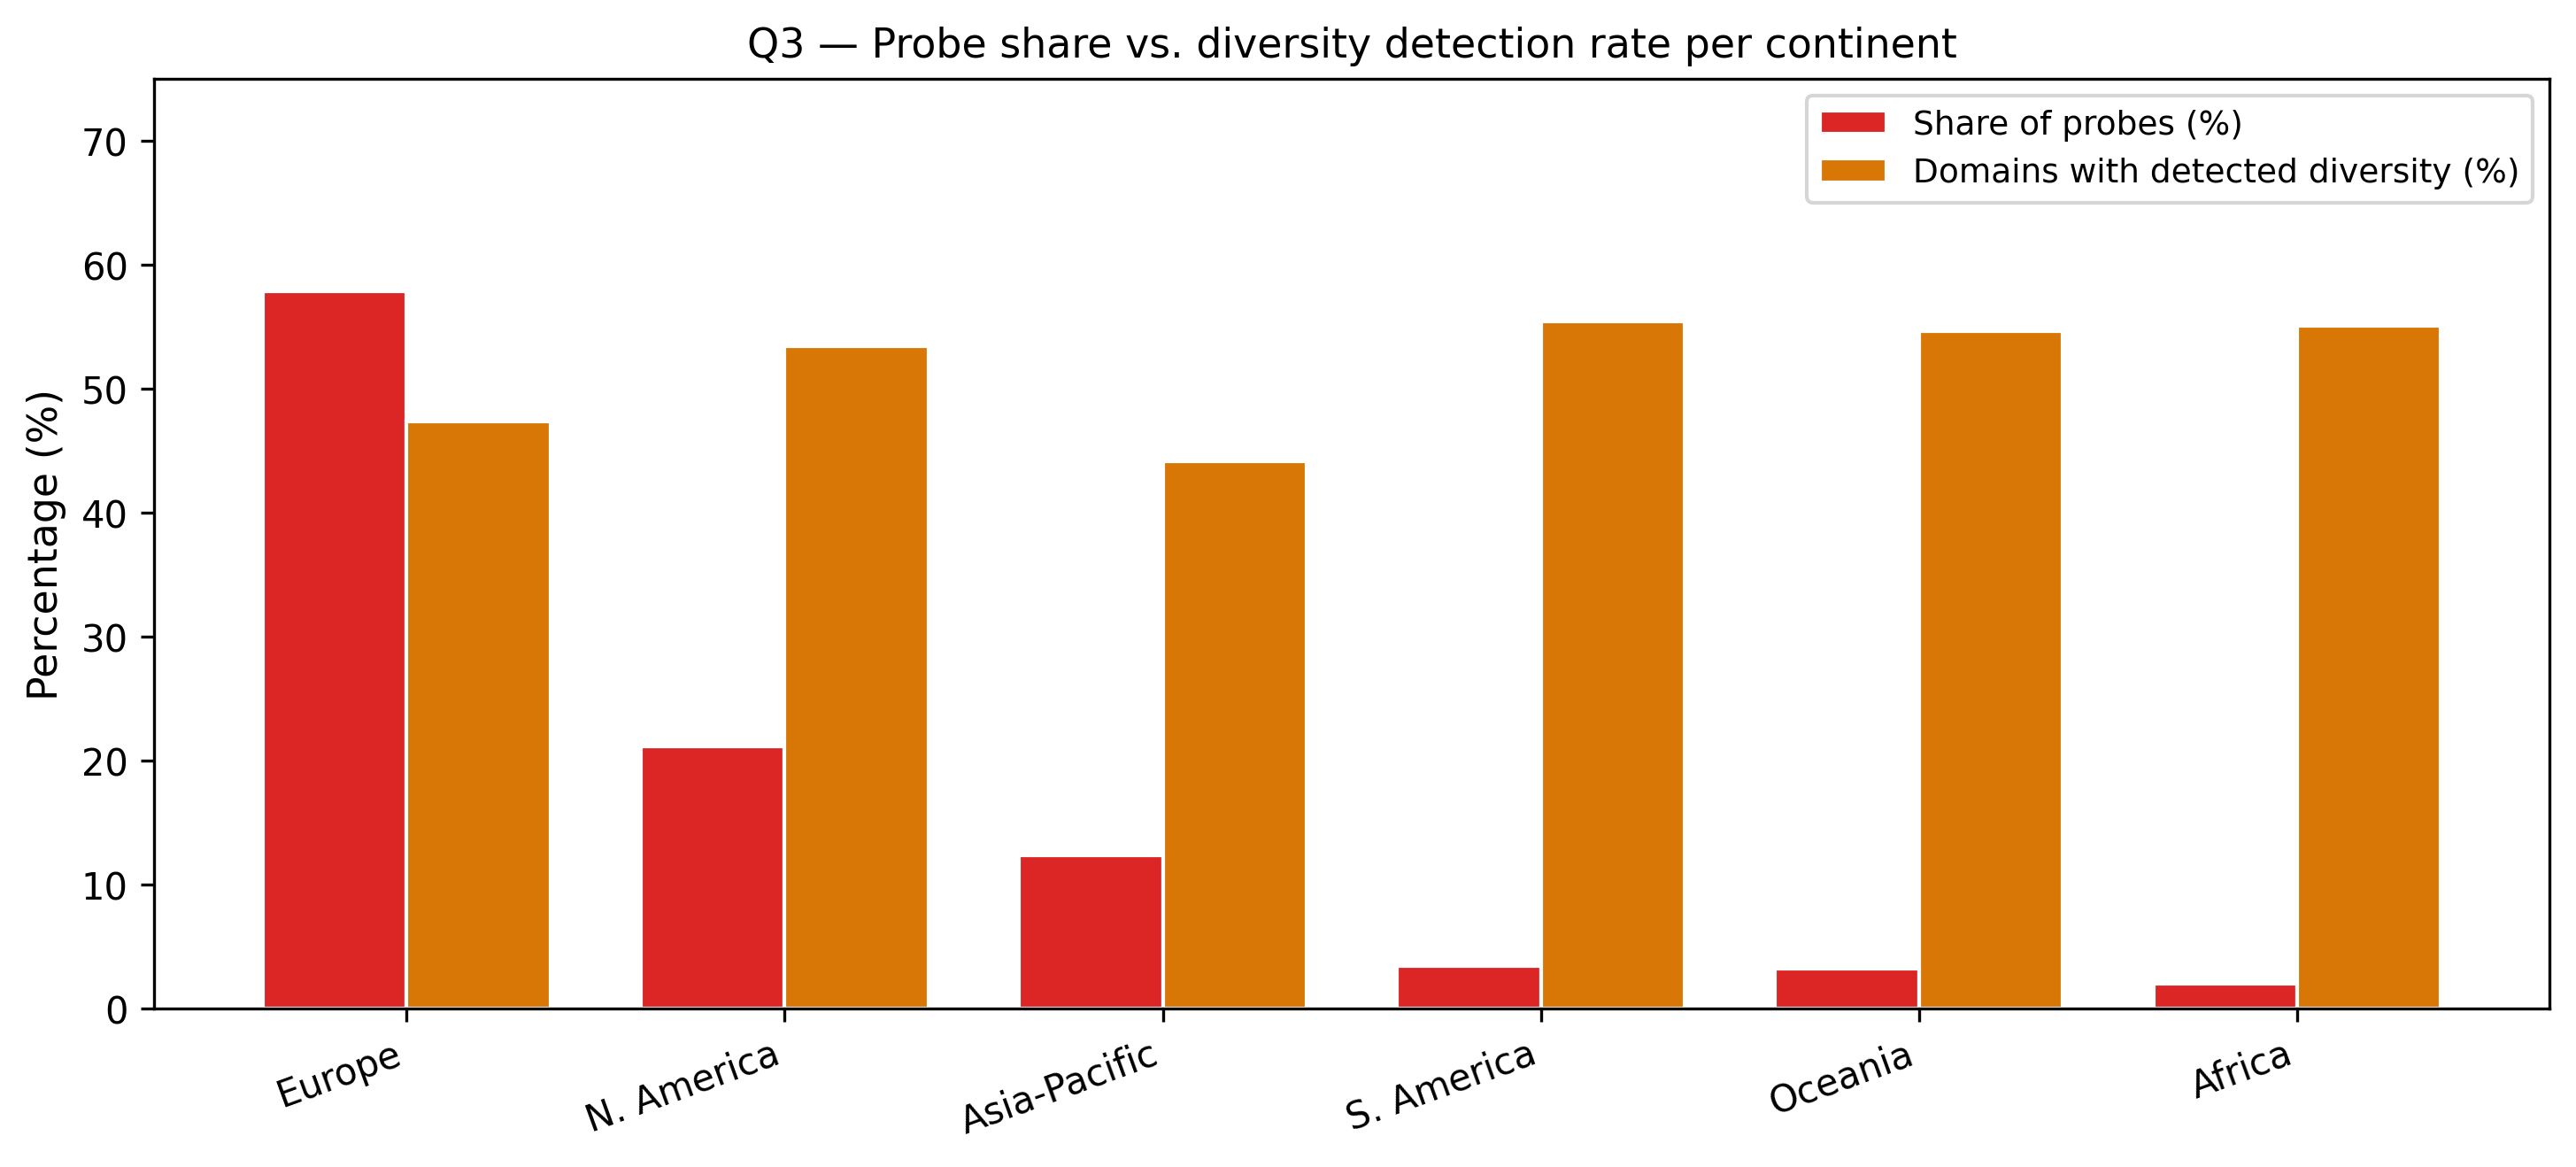
\includegraphics[width=\textwidth]{figures/fig_q3_probe_bias.png}
\caption{Probe share versus diversity detection rate per continent. Red bars show each continent's share of unique probe IDs in the dataset; orange bars show the percentage of domains for which that continent's probes detect at least one day of geographically differentiated \ac{DNS} responses. Despite holding only 2--3\% of probes, South America (58.3\%), Oceania (59.5\%), and Africa (59.5\%) detect diversity in a share comparable to or above Europe (52.6\%) and Asia-Pacific (47.4\%), which together hold 70\% of probes. This indicates that geographic probe imbalance does not prevent under-represented regions from contributing meaningful diversity observations.}
\label{fig:q3}
\end{figure}

\subsection{Interpretation}
\label{subsec:4.4.3}

Figure~\ref{fig:q3} reveals a counter-intuitive result: despite holding only 2--3\% of probes, South America (58.3\%), Oceania (59.5\%), and Africa (59.5\%) detect geographic \ac{DNS} diversity in a proportion of domains comparable to or above Europe (52.6\%) and Asia-Pacific (47.4\%), which together account for 70\% of probes. This finding suggests that probe density does not limit the ability to detect geographic diversity: even a small number of probes from an under-represented region is sufficient to observe that authoritative servers return different \ac{IP} addresses there. The Mann-Whitney test ($p = 0.091$) does not reach conventional significance, consistent with the absence of a statistically measurable difference between the EU+NA response distribution and that of other continents.

The practical implication for the 59.9\% geographic diversity rate reported in Section~\ref{sec:4.2} is nuanced: the rate is unlikely to be significantly biased downward by probe imbalance, since under-represented regions actively contribute diversity observations. The 99.6\% domain coverage per continent confirms that every region provides measurements for virtually every domain, avoiding the partial coverage problem that would make cross-continental comparisons unreliable.

\bigskip
\section{Results for Q4: Impact of Resolver Choice}
\label{sec:4.5}

\textbf{Research question}: Do the three major public \ac{DNS} resolvers (Google 8.8.8.8, Cloudflare 1.1.1.1, Quad9 9.9.9.9) return consistent \ac{DNS} responses for the same domain queried from the same geographic location, and how large is the inter-resolver divergence?

\subsection{Overview of the Q4 Campaign}
\label{subsec:4.5.1}

The Q4 campaign queried 250 domains using the same 200 RIPE Atlas probes as Q1--Q3, directing recursive \ac{DNS} queries to three public resolvers rather than to authoritative servers directly. The campaign was executed as a one-off measurement in June 2026 (measurements 177,787,616 to 179,470,557), comprising 750 individual RIPE Atlas measurements (250 domains $\times$ 3 resolvers). Each measurement targeted 200 probes, for a theoretical maximum of 50,000 probe-level results per resolver; the realised totals (Table~\ref{tab:q4_resolver_stats}) reflect a minor availability loss of 3--6\%.

\subsection{Per-Resolver Statistics}
\label{subsec:4.5.2}

\begin{table}[H]
\centering
\small
\begin{tabular}{l r r r r r}
\toprule
\textbf{Resolver} & \textbf{n (results)} & \textbf{Error rate} & \textbf{Avg RTT (ms)} & \textbf{Median RTT (ms)} & \textbf{Avg answers} \\
\midrule
Cloudflare (1.1.1.1) & 47{,}346 & 2\% & 45.8 & \textbf{15.5} & 2.27 \\
Google (8.8.8.8)     & 47{,}318 & 1\% & 50.5 & 24.7          & 2.25 \\
Quad9 (9.9.9.9)      & 47{,}067 & 1\% & 68.2 & 23.4          & 2.24 \\
\bottomrule
\end{tabular}
\caption{Q4 per-resolver statistics (250 domains, 200 probes, one-off campaign, June 2026)}
\label{tab:q4_resolver_stats}
\end{table}

Error rates are uniformly low across the three resolvers (1--2\%), confirming the availability reliability of these public services. The performance gap is more pronounced: Cloudflare's median \ac{RTT} of 15.5\,ms is 37\% lower than Google's (24.7\,ms) and 34\% lower than Quad9's (23.4\,ms). The mean \ac{RTT} values are substantially higher (45.8, 50.5, and 68.2\,ms respectively), reflecting the strongly right-skewed distribution caused by high-latency probes in Africa, Oceania, and South America. Figure~\ref{fig:q4a} illustrates both metrics.

\begin{figure}[H]
  \centering
  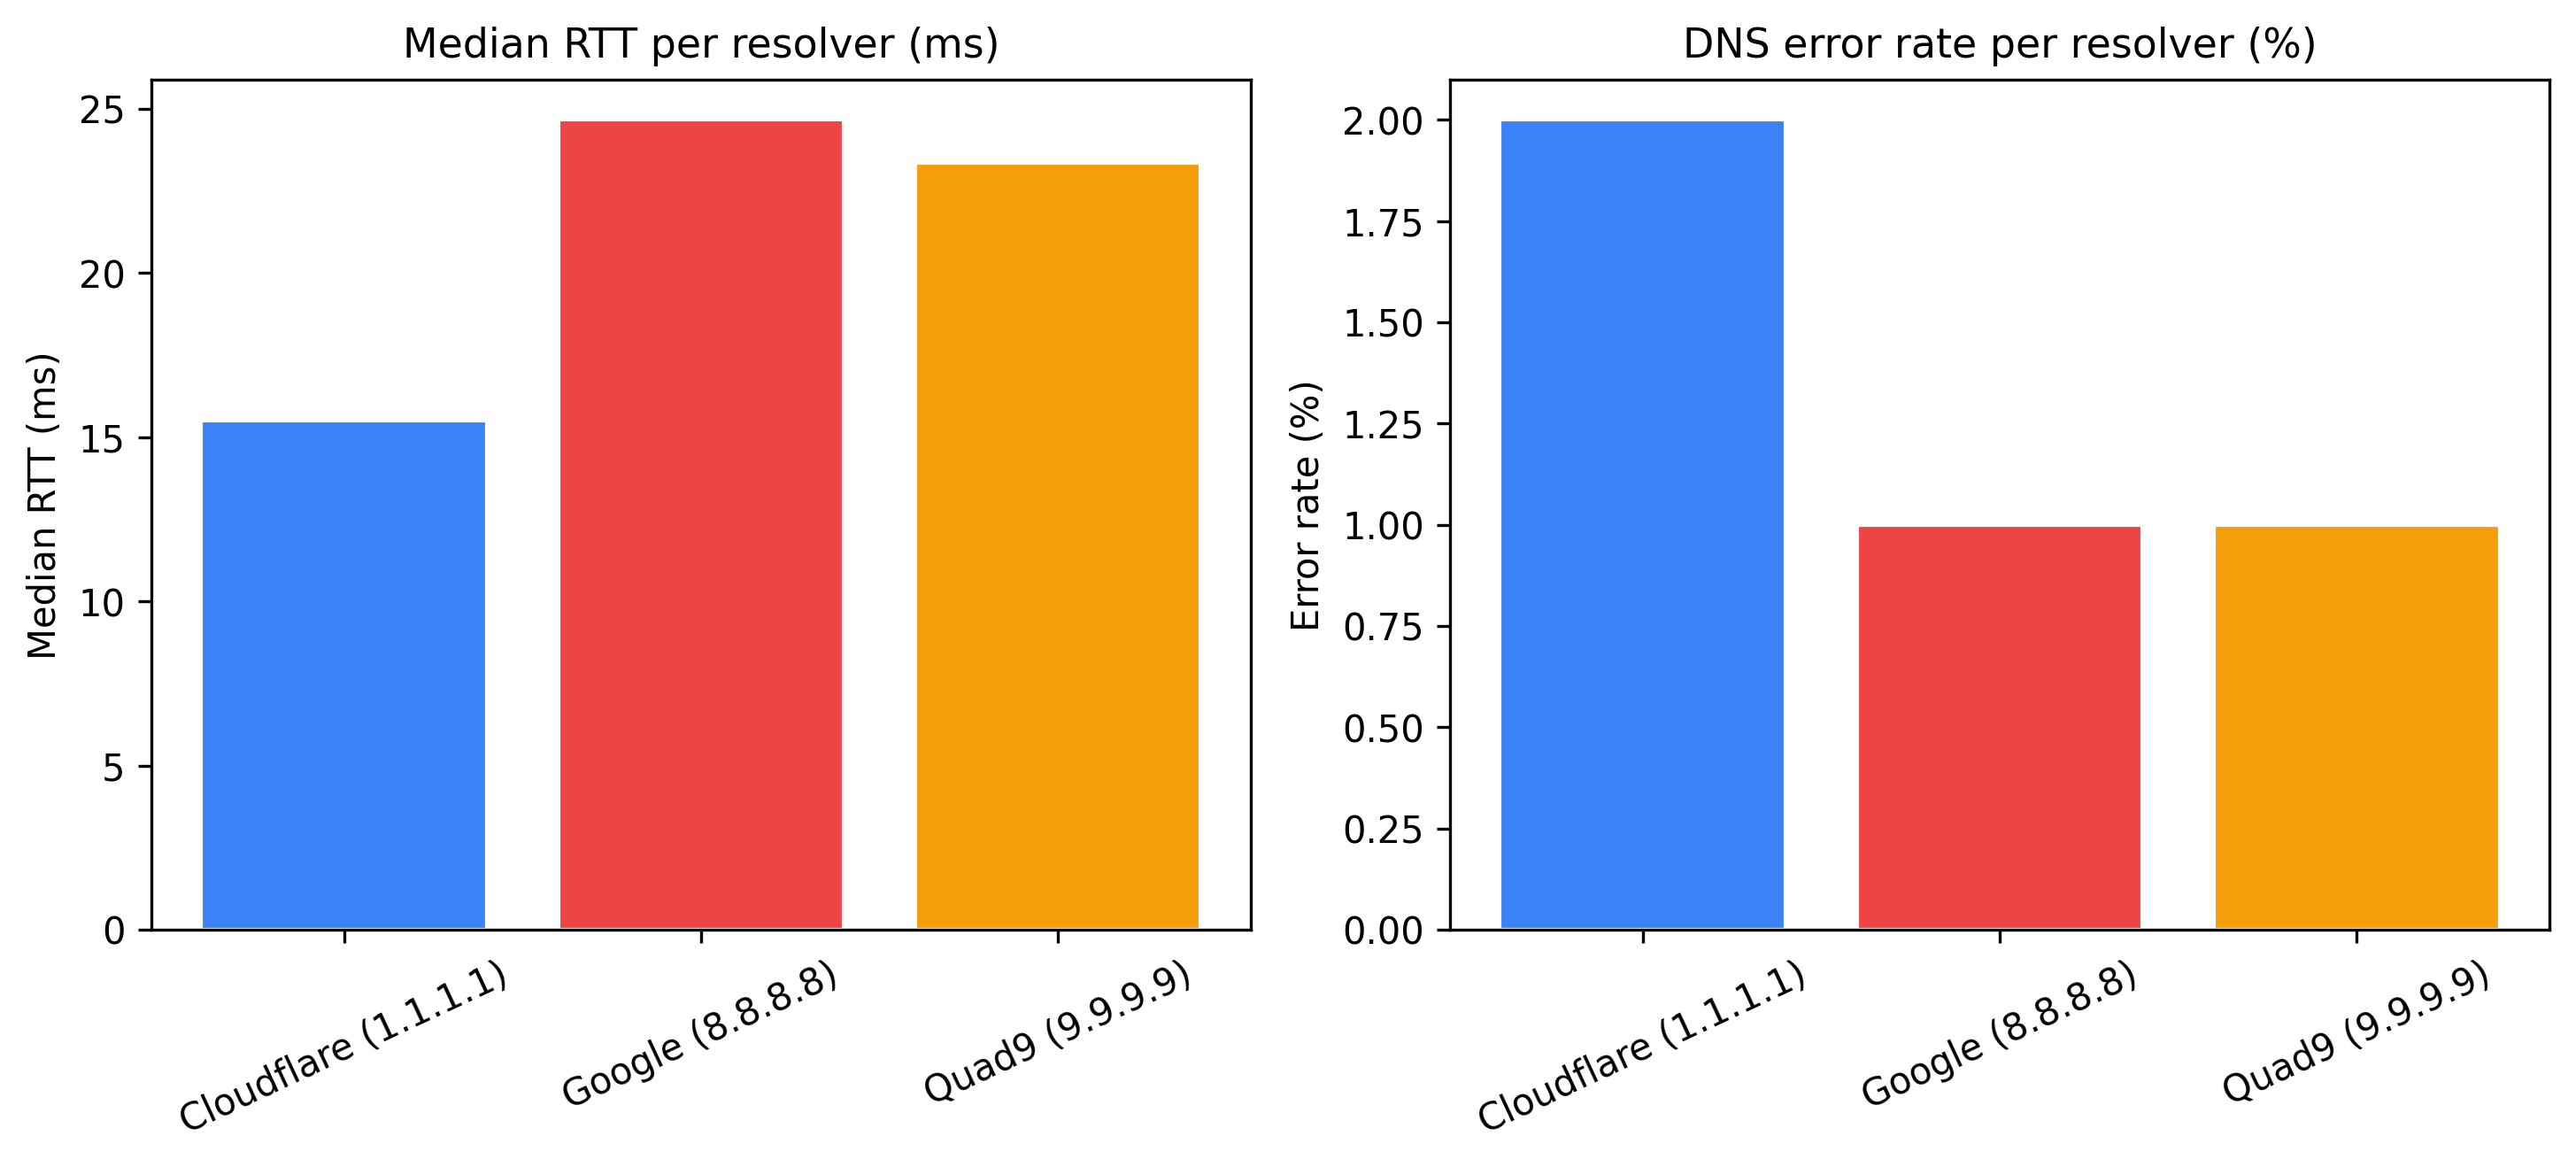
\includegraphics[width=0.92\textwidth]{figures/fig_q4_resolver_comparison.png}
  \caption{Q4 — Median RTT and error rate per public resolver (250 domains, 200 probes)}
  \label{fig:q4a}
\end{figure}

The mean answer count (2.24--2.27) is nearly identical across resolvers, indicating that all three retrieve the same number of \ac{IP} addresses for a given domain in expectation. The divergence analysis below clarifies whether those addresses are geographically equivalent.

\subsection{Cross-Resolver IP Divergence}
\label{subsec:4.5.3}

For each (domain, probe) pair with responses from all three resolvers, the returned \ac{IP} sets are compared pairwise. A divergence event is recorded when the two \ac{IP} sets are completely disjoint (no shared address). Table~\ref{tab:q4_divergence} reports the divergence rates for all three resolver pairs.

\begin{table}[H]
\centering
\small
\begin{tabular}{l r}
\toprule
\textbf{Resolver pair} & \textbf{Divergence rate (\% disjoint IP sets)} \\
\midrule
Cloudflare vs Google & 51.83\% \\
Cloudflare vs Quad9  & 52.81\% \\
Google vs Quad9      & 54.99\% \\
\bottomrule
\end{tabular}
\caption{Q4 cross-resolver \ac{IP} divergence: fraction of (domain, probe) pairs returning completely disjoint \ac{IP} sets}
\label{tab:q4_divergence}
\end{table}

More than half of all (domain, probe) observations yield entirely different \ac{IP} addresses depending on which public resolver is queried. The divergence rates are remarkably consistent across the three pairs (51--55\%), indicating that the phenomenon is not specific to any single resolver but is a structural property of the public \ac{DNS} resolution ecosystem. Figure~\ref{fig:q4b} visualises these rates.

\begin{figure}[H]
  \centering
  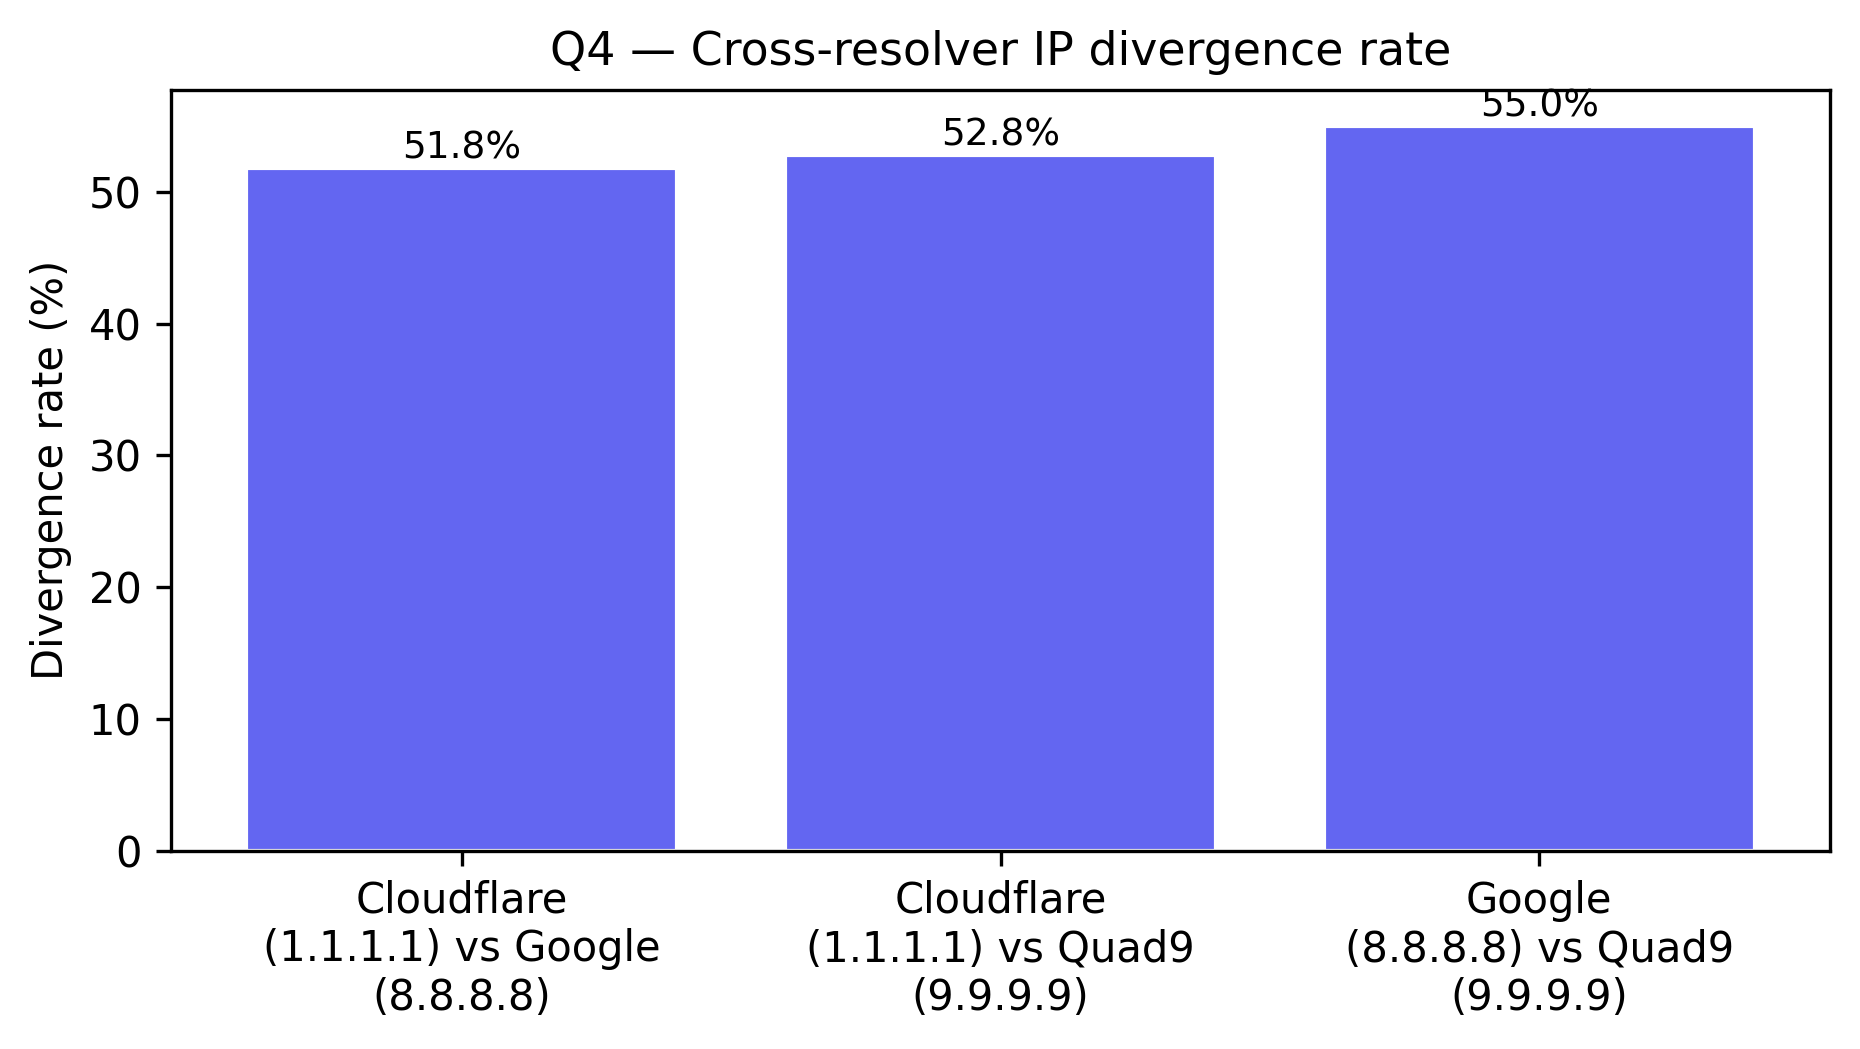
\includegraphics[width=0.72\textwidth]{figures/fig_q4b_divergence.png}
  \caption{Q4 — Cross-resolver \ac{IP} divergence rate: fraction of (domain, probe) pairs with completely disjoint \ac{IP} sets}
  \label{fig:q4b}
\end{figure}

Two mechanisms jointly explain this result. First, all three resolvers operate global anycast networks: Google 8.8.8.8, Cloudflare 1.1.1.1, and Quad9 9.9.9.9 each have hundreds of \ac{PoP}s worldwide with partially independent routing tables. A query from a given probe reaches whichever anycast instance wins the \ac{BGP} routing competition for that resolver's prefix. The winning instance forwards the query from its own \ac{IP} space, which \ac{CDN} authoritative servers use to assign a geographically optimised answer pool. Since different resolver anycast instances are co-located with different \ac{ISP}s and in different cities, the same probe may reach geographically distinct forwarding points depending on which resolver it queries, yielding different \ac{CDN}-assigned \ac{IP} pools.

Second, the three resolvers differ substantially in their \ac{EDNS} Client Subnet (\ac{ECS}) policies~\cite{RFC7871}: Cloudflare forwards the full client \ac{IP} prefix to authoritative servers by default, while Google forwards a /24 prefix, and Quad9 suppresses \ac{ECS} entirely for privacy. \ac{CDN} authoritative servers that implement \ac{ECS}-aware routing (a practice documented by Wang et al.~\cite{Wang2018} and Hours et al.~\cite{Hours2016}) therefore receive different geographic signals from the three resolvers and respond with different \ac{IP} pools for the same domain. The effect is especially pronounced for major \ac{CDN}-backed properties, which constitute the majority of the Tranco Top-250 corpus.

\bigskip
\section{Summary of Partial Results}
\label{sec:4.6}

\subsection{Answers to the Research Questions}
\label{subsec:4.6.1}

\textbf{Q1 --- Geographic diversity}: 59.9\% of Tranco Top 248 domains (148 of 247 analysed) return geographically differentiated \ac{DNS} responses at the continent level over the 50-day measurement campaign (based on 45-day partial data). At the country level, 60.3\% of domains (149 of 247) show differentiation. The mean number of distinct \ac{IP} address sets is 2.67 per domain at the continent level and 11.45 at the country level. The 77.3\% \ac{NSID} presence rate confirms that anycast-based authoritative \ac{DNS} deployment is the predominant infrastructure mechanism.

\textbf{Q2 --- Temporal stability}: The daily \ac{DNS} response change rate is 38.24\%, and the weekly (38.29\%) and monthly (38.30\%) rates are nearly identical across 44, 38, and 15 pairs respectively (45-day partial data; final dataset will yield approximately 49, 43, and 20 pairs), confirming a stationary churn process driven by \ac{CDN} pool rotation. Of 247 domains, 20.6\% are fully stable; the median per-domain change rate is 48.8\%.

\textbf{Q3 --- RIPE Atlas geographic bias}: The actual probe distribution (EU 57.8\%, NA 21.2\%, AP 12.4\%, SA 3.4\%, OC 3.2\%, AF 2.0\%) is heavily concentrated in Europe and North America (79.0\% combined). A Mann-Whitney U test yields $U = 256{,}971.5$, $p = 0.091$, above the $\alpha = 0.05$ significance threshold. Crucially, under-represented continents --- Africa (59.5\%), South America (58.3\%), and Oceania (59.5\%) --- each detect geographic diversity in more than 58\% of domains despite holding only 2--3\% of probes, at or above the Europe rate (52.6\%), indicating that the zone-based probe assignment preserves diversity observability across all regions.

\textbf{Q4 --- Resolver impact}: The three public resolvers show low and consistent error rates (1--2\%) but significantly different latency profiles: Cloudflare's median \ac{RTT} of 15.5\,ms is 37\% lower than Google (24.7\,ms) and Quad9 (23.4\,ms). More strikingly, the cross-resolver \ac{IP} divergence rate exceeds 50\% for all three resolver pairs (51.8\%–55.0\%), meaning that for more than half of (domain, probe) observations, two public resolvers return completely different \ac{IP} addresses for the same domain from the same location. This is driven by both anycast routing differences and divergent \ac{ECS} policies between resolvers.

\subsection{Result Limitations}
\label{subsec:4.6.2}

The results presented in this chapter are subject to the following constraints:

\begin{itemize}
  \item \textbf{Measurement duration}: The 50-day campaign (2 April -- 21 May 2026) will yield approximately 49 daily pairs, 43 weekly pairs, and 20 monthly comparison pairs for Q2. The 45-day partial dataset already provides reliable estimates across all three windows; the monthly estimate of 38.30\% rests on fifteen pairs and is well-established.
  \item \textbf{Phase transition}: The first nine days (pilot) used 99 domains and 50 probes; the following 41 days of the main phase (11 April -- 21 May 2026) use 248 domains and 200 probes. Analyses covering the mixed 45-day window combine these two experimental conditions; domain-level results are consistent because the main-phase corpus is a superset of the pilot corpus, but probe-count differences may affect per-domain diversity estimates.
  \item \textbf{Platform bias}: Despite geographic stratification, RIPE Atlas probe coverage remains heavily concentrated in Europe (57.8\%). The Q3 analysis shows that this imbalance does not prevent under-represented regions from detecting geographic diversity, but the lower probe density in Africa, South America, and Oceania reduces within-region statistical reliability (higher variance per single-probe country).
  \item \textbf{Domain coverage}: The analysis covers the Tranco Top 250 only. Of the 250 domains in the corpus, 2 were excluded during pre-validation because their authoritative name server \ac{IP} address could not be resolved (see Section~\ref{subsec:3.2.3}), leaving 248 active RIPE Atlas measurements. A further domain produced no valid results during the campaign and was excluded from analysis, resulting in a final corpus of 247 domains.
  \item \textbf{\ac{IPv4} only}: All measurements query \ac{DNS} \ac{A} records over \ac{IPv4}. \ac{AAAA} records and \ac{IPv6} transport are not covered. \ac{IPv6} \ac{CDN} deployment may exhibit different geographic routing patterns, and the results presented here do not characterise the \ac{IPv6} \ac{DNS} landscape.
\end{itemize}
